% !TEX root = ./HY-CS-main.tex
\chapter{Oppimisen analysoinnin tarpeet\label{oppimisenanalysoinnintarpeet}}

Oppimisanalytiikka haluaa tutkia oppimista ja opettamista oppimisympäristöissä ja yrittää hyödyntää analytiikkaa tunnistaessaan poikkeamia tai tehdessään muita oppijaa tukevia havaintoja \citep{longPenetratingFogAnalytics2011}. Vakiintunut oppimisanalytiikan määritelmä on 1st International Conference on Learning Analyticsin määritelmä \citep{siemensLearningAnalyticsEmergence2013}. Sen mukaan oppimisanalytiikka on oppijoista kerättävän datan mittaamista, keräämistä, analysointia ja raportointia, jota hyödynnetään oppimisen ja sen ympäristön ymmärtämiseen ja optimoimiseen \citep{clowLearningAnalyticsCycle2012}.


\section{Oppimisanalytiikka pedagogisena työkaluna}

Oppimisanalytiikaa voidaan hyödyntää kolmessa eri käyttötarkoituksessa, joita ovat kuvaileva analytiikka, ohjaava analytiikka ja ennustava analytiikka \citep{auvinenOppimisanalytiikkaTuleeOletko2017, danielBigDataAnalytics2015}. Analyyttiset mallit ovat tämän kolmijaon keskiössä. Kuvailevassa analytiikassa kuvaillaan ja analysoidaan oppijoista sekä muista oppimisen osa-alueista saatavaa historiatietoa. Kuvaileva analytiikka etsii esimerkiksi nykyisiä oppimistrendejä. Ennustava analytiikka puolestaan tarjoaa oppilaitoksille mahdollisuuden tehdä datan perusteella parempia päätöksiä ja näkymiä nykytilasta. Tavoitteena on estimoida tulevien tapahtumien todennäköisyyksiä. Ohjaava analytiikka puolestaan tarjoaa oppilaitoksille mahdollisuuden arvioida nykyistä toimintaansa vaihtoehtoisten mallien pohjalta ja ohjaa parempiin päätöksiin.

Oppimisanalytiikkaa voidaan kuvata kiertävänä syklinä \citep{clowLearningAnalyticsCycle2012}. Syklissä on neljä kohtaa: oppija, data, analyysi ja toiminta. Kuitenkaan aina kaikki neljä osa-aluetta eivät ole mukana, vaikka prosessi olisi oppimisanalytiikkaa. Esimerkki tälläisestä prosessista on raporttien muodostaminen, mutta tämän pohjalta ei tehdä mitään toimenpiteitä.

\begin{figure}[h]
    \centering
    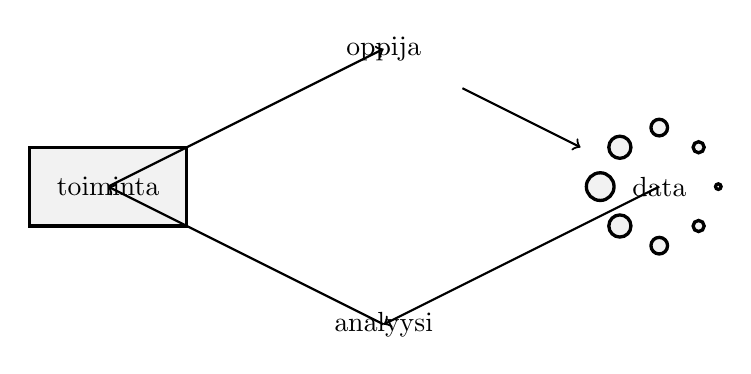
\begin{tikzpicture}
        \filldraw[color=black, fill=black!5, very thick] (-4.5,-0.5) rectangle (-2.5,0.5);

        \filldraw[color=black, fill=black!5, very thick] (4,0.5) circle (2pt);
        \filldraw[color=black, fill=black!5, very thick] (3.5,0.75) circle (3pt);
        \filldraw[color=black, fill=black!5, very thick] (3,0.5) circle (4pt);

        \filldraw[color=black, fill=black!5, very thick] (4,-0.5) circle (2pt);
        \filldraw[color=black, fill=black!5, very thick] (3.5,-0.75) circle (3pt);
        \filldraw[color=black, fill=black!5, very thick] (3,-0.5) circle (4pt);

        \filldraw[color=black, fill=black!5, very thick] (2.75,0) circle (5pt);
        \filldraw[color=black, fill=black!5, very thick] (4.25,0) circle (1pt);

        \node[] at (0,1.75) {oppija};
        \node[] at (3.5,0) {data};
        \node[] at (0,-1.75) {analyysi};
        \node[] at (-3.5,0) {toiminta};


        \draw[thick, ->] (1,1.25) -- (2.5,0.5);
        \draw[thick, ->] (3.5,0) -- (0,-1.75);
        \draw[thick, ->] (0,-1.75) -- (-3.5,0);
        \draw[thick, ->] (-3.5,0) -- (0,1.75);
    \end{tikzpicture}
    \caption{Oppimisanalytiikan eri vaiheet tiivistetysti \citep{clowLearningAnalyticsCycle2012}.}
\end{figure}

Syklissä oppija on oppimisanalytiikan lähtökohta \citep{clowLearningAnalyticsCycle2012}. Oppijoista kerätään dataa \citep{wolffImprovingRetentionPredicting2013}, joka on analyiikan lähtökohta. Data koostuu oppijoiden toiminnasta esimerkiksi verkko-oppimisympäristössä tai opintotietojärjestelmätiedosta. Oppimisympäristöstä saatavaa dataa voi olla esimerkiksi lokeihin jäänyt tieto oppijan oppimisympäristössä liikkumisesta tai opintotietojärjestelmässä aiemmat kurssisuoritukset. Toisaalta myös oppijan oppimiskäyttäytymisen ja -tyylin ymmärtäminen ovat oppimisanalytiikassa keskistä \citep{hasanPredictingStudentPerformance2020}.

Oppijasta muodostunutta dataa voidaan tarkastella ja analysoida havainnollistaaksemme oppimisprosessia \citep{clowLearningAnalyticsCycle2012}. Tämä on oppimisanalytiikan tärkein vaihe, jossa muodostetaan prosessista saatava lisäarvo. Oppijoista saatavan datan perusteella voidaan tunnistaa esimerkiksi putoamisvaarassa olevia opiskelijoita tai ennustaa heidän menestymistä kurssilla.

Oppimisanalytiikassa syklin viimeinen kohta, toiminta, on merkittävässä roolissa \citep{clowLearningAnalyticsCycle2012}. Toiminnan tarkoitus on vaikuttaa oppijaan. Toimintaa voi olla esimerkiksi oppijan käytössä oleva seurantanäkymä, jossa voi vertailla toisiin opiskelijoihin tai tarvittavan tuen kartoittaminen putoamisvaarassa olevalle opiskelijalle. Oppija voi hyödyntää analytiikasta saatavaa tietoa oman oppimisensa kehittämiseen hyvin nopeallakin vasteajalla ja vaikutukset kohdistuvat oppijaan itseensä.

Aina toiminta ei tavoita oppijaa, sillä tuloksia voidaan hyödyntää usealla tasolla \citep{clowLearningAnalyticsCycle2012}. Opettaja voi hyödyntää aiemman kurssi-iteraation kurssiarvosanoja kurssin kehittämisen tukena. Kurssin aikana opettajat toimet voivat vaikuttaa yhden oppijan sijasta myös useampaan oppijaan, ja opettajan toiminnan vaikutukset eivät välttämättä ole heti havaittavissa.

Hallintohenkilöstön toiminnan vaikutukset ovat laajempia ja hitaammin havaittavia heidän yhdistäessä myös opettajalta saatavan palautteen analyysiinsa \citep{clowLearningAnalyticsCycle2012}. Hallintohenkilöstö pystyy toiminnallaan vaikuttamaan isompaan joukkoon oppijoita kuin yksittäinen oppija, kuten jakamalla kurssin kahteen osaan. Toisaalta oppimisanalytiikkaa voidaan hyödyntää laajemmalla tasolla esimerkiksi osana opetussuunnitelmatyötä, jolloin vaikutukset ovat vielä hitaammin havaittavissa, mutta niiden kattavuus on laajin. \citep{clowOverviewLearningAnalytics2013}

Oppimisanalytiikkaa voidaan hyödyntää usealla eri tasolla \citep{longPenetratingFogAnalytics2011,siemensLearningAnalyticsEmergence2013}. Kurssitasolla voidaan seurata opiskelijan toimintaa kurssilla ja tehdä havaintoja kurssin edistymisestä sekä sillä menestymisestä. Tätä voidaan tehdä esimerkiksi luokittelulla tai ennustavilla malleilla riippuen mitä halutaan analysoida. Yksi taso on hyödyntää oppimisanalytiikkaa sisällön suosittelemiseen. Tässä oppijan oppimispolku muotoillaan osaamista vastaavaksi esimerkiksi ohjaamalla perusasiat jo hyvin osaava oppija haasteellisemmalle kurssille tai tarjotaan heikommin pärjäävälle opiskelijalle taitotasoa vastaavia tehtäviä. \color{red}(HOX! Tsiikaa noi muut kolme muuta Longin nostoa sekä table 1)\color{black}

\section{Moodle datalähteenä}

Moodle (Modular Object-Oriented Dynamic Learning System) on vuodesta 1999 lähtien kehittetty avoimen lähdekoodin verkko-oppimisympäristö, joka on julkaistu GPL-3.0 -lisenssillä \citep{dougiamasPowerOpenEducational2021,dougiamasMoodle2022}. Moodlella on yli 315 miljoonaa käyttäjää eri puolilla maailmaa 178 tuhannella eri Moodle-sivustolla \citep{moodle.orgMoodleStatistics}. Moodle on rakennettu käyttäen ohjelmointikielenä PHP:tä ja tiedon tallentamiseen relaatiotietokantaa. Suorat SQL-kyselyt tietokantaan ja Moodlen tarjoamat metodit mahdollistavat Moodlen keräämän tiedon hyödyntämisen osana data-analyysia. Moodlen tietokantarakenteesta löytyy selkeä indeksointi avaimien perusteella \citep{greenMoodle11Database2022}, jonka perusteella tietokantataulusta toiseen asioiden jäljittäminen on mahdollista.

Moodle tallentaa tietokantatauluun \emph{logstore\_standard\_log} kaikki Moodlen Event API:n kautta tulevat tapahtumat \citep{dougiamasMoodle2022, dougiamasLoggingMoodleDocs2021}. Tapahtumien avulla voidaan kerätä tietoa toiminnasta verkko-oppimisympäristössä \citep{agudo-peregrinaCanWePredict2014}. Lokitietoa erilaisista tapahtumista voi esimerkiksi tulla Moodlen ytimen komponenteista, eri aktiviteeteistä, työkaluista ja raporteista riippuen komponentin luonteesta. Useimmat aktiviteetit tallentavat lokiin merkittäviä tapahtumia, kuten suorituksien luomisen aktiviteettiin, kurssimoduulissa vierailun, tenttiin vastaamisen ja vertaisarvioinnin antamisen. Moodlen ytimessä oppijan kannalta tärkeimmät ovat kirjautumiseen ja kurssin katseluun liittyvät tapahtumat. Lokitietoihin tallentuu aina tieto kuka on vieraillut, milloin on vieraillut, missä on vieraillut ja mistä on vieraillut \citep{abdullahLearningStyleClassification2015}. Tapahtumalokin avulla voidaan tarkastella oppijoiden toiminnan painottumista eri kellonaikoihin.

Moodlessa on vakiona 23 erilaista aktiviteettiä, joista jokainen tallentaa erilaista tietoa tietokantaan \citep{dougiamasMoodle2022}. Jokaisella aktiviteetillä on myös omia tietokantatauluja, joihin tallennetaan aktiviteettiin liittyvä tieto. Lisäksi Moodlen kehittäjäyhteisö on julkaissut paljon Moodlea laajentavia aktiveettejä \citep{moodle.orgMoodlePluginsDirectory2022}. Oppilaan osaamista mittaavia aktiviteettejä ovat esimerkiksi tentti, palaute, työpaja, oppitunti, keskustelualue ja H5P. Esimerkiksi työpaja tallentaa kaikki suoritukset tauluun \emph{workshop\_submissions} ja suorituksien arvioinnit tauluun \emph{workshop\_grades} \citep{greenMoodle11Database2022}. Työpaja mahdollistaa myös vertaisarvioinnin (taulussa \emph{workshop\_assessments}), jossa oppija joutuu arvioimaan omaa ja toisten osaamista hyödyntämisen analytiikassa. Keskustelualueelta voidaan mitata oppijoiden aktiivisuutta viestien lukumäärällä \citep{mwalumbweUsingLearningAnalytics2017}. Aktiviteetistä myös saadaan tieto, onko sitä avattu kertaakaan taulusta \emph{course\_module\_completion}.

Moodlen yhteisö on myös etsinyt erilaisia tapoja kerätä palautetta oppijoilta. Yksi tälläinen on pikapalautetoiminnallisuus (block\_point\_view), joka antaa kolmiportaisen itsearviointimahdollisuuden aktiviteettikohtaisesti \citep{fombaronMoodlePluginPoint2021}. Tämä mahdollistaa helpon ja nopean tavan saada oppijalta itsearviointidataa siitä, miten oppija itse näkee oman suoriutumisensa kyseisessä tehtävässä. Tietokantataulusta \emph{block\_point\_view} pystytään hakemaan käyttäjän äänestystulos kurssin, kurssimoduulin tai käyttäjän perusteella.

Joidenkin tietojen, kuten oppijan tarkemman toiminnan seuraamiseen sivulla tarvitaan kolmannen osapuolen tuottamaa tekniikkaa \citep{filvaGoogleAnalyticsTime2014}. Tälläinen seuraamiseen soveltuva työkalu on esimerkiksi Google Analytics, joka seuraa tarkemmin käyttäjän toimintaa sivustolla. Moodlen lokitiedoista selviää milloin sivu on ladattu, mutta tietoa kuinka kauan oppija sivulla on todellisuudessa viettänyt aikaa ei tällä menetelmällä saada \citep{dougiamasMoodle2022}. On teoreettisesti mahdollista, että oppija on avattuaan sivun katsellut sitä minuutin ajan ja tämän jälkeen lähtenyt kahville. Jos seuraava sivulataus on tunnin päästä, niin tästä ei pystytä luotettavasti laskemaan sivulla vietettyä todellista aikaa.

Learning Analytics API tarjoaa Moodlen oman rajapinnan oppimisanalytiikan toteuttamiseen \citep{oliveSupervisedLearningFramework2018}. Moodlessa se jakautuu kahteen osaan, Moodlen Analytics API:n ja Machine Learning backendiin. Analytics API tuottaa mallien tarvitsemaa tietoa koneluettavassa CSV-muodossa. Backend puolestaan vastaa itse tiedon käsittelystä ja analysoinnista. Moodleen on sisäänrakennettu tämän viitekehyksen sisällä opiskelijoiden tippumisen tunnistamisen tarjoava malli sekä kurssin opetuksen puuttumisen tunnistava malli \citep{monllaoAnalyticsAPIMoodleDocs2021}.

\section{Päättelymahdollisuudet}

Oppijan menestymistä kurssilla voidaan ennustaa eri tarkoituksissa \citep{barberCourseCorrectionUsing2012a}. Tähän voidaan hyödyntää aiempien kurssien menestystietoa muista lähteistä, sekä kurssin edistyessä lisätä kurssisuorituksista saatavaa tietoa mukaan analyysiin. Yhdistämällä tämän visualisointiin, voidaan tarjota oppijalle reaaliaikainen näkymä kurssiarvosanasta ja hyödyntää tätä motivaattorina. Yksi ennustamisen mahdollisuus on tarkastella valmistuuko koulutukseen hakija ennusteen mukaan tavoiteaikataulussa.

Toisaalta voidaan tarkastella onko oppija vaarassa pudota kurssilta \citep{oliveSupervisedLearningFramework2018, suhonenUsingMoodleData2019}. Tarkastellaan oppijan toimintaa verkko-oppimisympäristössä ja yritetään löytää eri merkkejä oppijan putoamisest akurssilta. Tarkastelua voidaan laajentaa myös kurssien väliseksi \citep{kinnari-korpelaOppimisanalytiikallaTehokkaampaanOhjaukseen2020} ja analytiikan löytäessä putoamisvaarassa olevan oppijan, voidaan hänelle tarjota kohdistetusti tukea oppimiseen jo aikaisessa vaiheessa.
% Etsi tämän lähde jostain: Paras tapa tunnistaa oppijan mahdollinen putoaminen on vertailla oppijan aiempaan käyttäytymiseen ja tunnistaa muutoksen merkkejä siinä (tälle oli kiva lähde, löytynee luvusta 3 :D).

Oppimisanalytiikan avulla voidaan tehdä opetuksen kehttämistä \citep{romeroEducationalDataMining2010}. Oppimisanalytiikasta saatavalla datalla voidaan suunnitella kurssien resursointia, kehittää opetussuunnitelmia sekä tukea hallinnon päätöksiä. Oppimisanalytiikalla voidaan löytää nykyisistä kursseista heikkoja kohtia, joihin ratkaisu voi olla esimerkiksi uuden kurssin luominen tai nykyisen kehittäminen tukemaan osaamisvajeen paikkaamista. Tämä voi näkyä esimerkiksi oppimateriaalin kehittämisenä, mikäli analytiikka osoittaa tietyn osa-alueen tehtävien menevän muita heikommin, kun saman aikaisesti tiettyä opetusmateriaalin osaa tarkastellaan muita enemmän.

Oppimispolku on ohjeistus, joka kertoo oppimistehtävien ohjeistukset ja tavoitteet, sekä havainnollistaa oppimisen edistymistä kurssin aikana \citep{toivolaFlippedLearningKaanteinen2017}. Oppimispolun halutaan mahdollistaa oppijan oman luontaisen oppimistahdin hyödyntäminen. Oppimisanalytiikan avulla voidaan visualisoida oppijan edistyminen oppimispolulla ja tarjota myös suosituksia seuraavista tehtävistä \citep{longPenetratingFogAnalytics2011}. Jos oppija ei ole vielä ymmärtänyt jotain oppimispolun osa-aluetta, voi analytiikka ehdottaa lisätehtävää osaamisen vahvistamiseksi ennen seuraavaan osa-alueeseen siirtymistä. Pikapalautetta voidaan hyödyntää itsearvioiden toteuttamiseen ja edelleen analytiikan tukena.

Tätä voitaisiin myös hyödyntää kurssipolkujen suunnittelussa ehdottamalla esimerkiksi oppijalle seuraavia kursseja aiempien kurssien menestyksen pohjalta \citep{longPenetratingFogAnalytics2011}. Jos oppija ei ole esimerkiksi pärjännyt matriisilaskennan ensimmäisellä kurssilla, niin oppimisanalytiikka voisi ehdottaa matriisilaskennan ensimmäisen kurssin asioita kertaavaa kurssia ennen siirtymistä toiselle kurssille.
